\documentclass[11pt]{article}

\usepackage[T1]{fontenc}
\usepackage[margin=1in]{geometry}
\usepackage[hypertexnames=false,hidelinks]{hyperref}
\usepackage{url}
\usepackage{booktabs}
\usepackage{amsfonts}
\usepackage{nicefrac}
\usepackage{microtype}
\usepackage{xcolor}
\usepackage{graphicx}
\usepackage{amsmath}
\usepackage{amssymb}
\usepackage{mathtools}
\usepackage{amsthm}
\usepackage{algorithm}
\usepackage{algorithmic}
\usepackage[square,numbers,sort&compress]{natbib}
\usepackage{titlesec}
\usepackage[capitalize]{cleveref}

\title{Charge-self-consistent equivariant potentials\\ for energetic molecular crystals: static gains and nonequilibrium limits}

\author{%
  Xiaohua Liu$^{a}$\thanks{Corresponding author: \texttt{xiaohualiu@jhun.edu.cn}}
  \and
  Dongping Chen$^{b}$
  \and
  Chengkai Zhang$^{a}$
  \and
  Hongqian Sang$^{a}$ \\
  $^{a}$\parbox{0.42\textwidth}{\centering State Key Laboratory of Precision Blasting,\\ Jianghan University, Wuhan 430056, Hubei, China}
  \hfill
  $^{b}$\parbox{0.42\textwidth}{\centering State Key Laboratory of Explosion Science and Safety Protection,\\ Beijing Institute of Technology, Beijing 100081, China} \\
}

\date{}

\setlength{\parindent}{1.2em}
\setlength{\parskip}{0.35em}
\linespread{1.05}
\setlength{\bibsep}{2pt}
\titleformat{\section}{\large\bfseries}{\thesection.}{0.5em}{}
\titleformat{\subsection}{\normalsize\bfseries}{\thesubsection.}{0.5em}{}

\hbadness=10000
\vbadness=10000
\hfuzz=30pt
\vfuzz=20pt
\emergencystretch=2em

\begin{document}

\maketitle

\begin{abstract}
Energetic molecular crystals provide a stringent test for machine-learned interatomic potentials because compression couples polarization, intermolecular rearrangement, and bond reorganization on short time scales. We introduce CSC-MACE, a charge-self-consistent extension of MACE that embeds differentiable charge equilibration within one periodic total-energy model. Across OpenREACT, Transition1x, SPICE, and CL-20/HMX, charge-aware effects are measurable but not uniformly beneficial. On the final CL-20/HMX target, the static ordering remains favorable under four held-out views, including a stronger temperature-gap block holdout: charge-aware models outperform the short-range baseline, and the \texttt{self\_consistent} branch achieves the lowest energy error while force accuracy remains effectively tied across families. Nonequilibrium behavior remains largely frame-dominated. A denser fragile-window analysis nevertheless reveals a narrow endpoint-survival gain on frames $64$--$72$. Explicit electrostatic response therefore improves static energetics on the energetic-material target, while dynamic gains remain confined to a narrow local endpoint-survival window rather than a robust nonequilibrium hierarchy.
\end{abstract}

\section{Introduction}
Energetic molecular crystals such as CL-20 and HMX remain a difficult regime for atomistic simulation because compression, intermolecular rearrangement, bond breaking, and charge redistribution unfold on comparable femto--picosecond time scales. In that setting, a potential must remain reliable not only near equilibrium, but also for distorted configurations in which polarization and changing molecular environments can alter both relative energetics and subsequent trajectory evolution \cite{valeeswaran2023charge,menikoff2016shock,bolton2008molecular}.

Recent machine-learned interatomic potentials have substantially improved the accuracy and scale of atomistic simulation, particularly through equivariant architectures that encode geometric symmetry directly \cite{batatia2022mace,batzner20223,musaelian2023learning,liao2023equiformer,batatia2023foundation}. At the same time, recent reviews and transferability studies have made clear that accuracy, transfer, and execution cost remain tightly coupled design constraints rather than independent objectives \cite{musil2021physics,unke2021machine,goedecker2023perspective,jacobs2025practical,huang2025cross}.

For reactive molecular crystals, a central ambiguity therefore remains. When a finite-cutoff model fails under compression or along nonequilibrium trajectories, the missing ingredient may be a richer short-range representation, but it may equally be an explicit treatment of environment-dependent electrostatic response. That distinction is especially important for energetic materials, where polarization and charge transfer have long been implicated in sensitivity, decomposition, and shock response \cite{valeeswaran2023charge,van2001reaxff}.

Charge-aware machine-learning potentials offer a natural route toward that missing physics. Charge-equilibration ideas originate in the QEq formalism of Rapp\'e and Goddard \cite{rappe1991charge} and now appear in several atomistic-learning frameworks that couple learned local features to environment-dependent charges or electrostatic observables \cite{gastegger2017machine,unke2019physnet,ko2021fourth,fuchs2025celli}. Contemporary materials studies have also begun to test such ideas directly under non-equilibrium conditions. The question is therefore no longer whether long-range response can be embedded in an MLIP, but how that response changes structural stability once trajectories leave the near-equilibrium manifold \cite{jung2026charge}.

What remains unresolved is whether explicit charge self-consistency improves the observables that matter most for energetic-material modelling. A better electrostatic description may sharpen static energy ranking without stabilizing the nonequilibrium quantities that govern bond survival, fragment integrity, and trajectory degradation. The relevant question is therefore not simply whether charge-aware models lower a benchmark error, but whether they alter the failure structure of trajectories that are already leaving the near-equilibrium manifold.

We address that question with CSC-MACE, a charge-self-consistent extension of MACE in which equivariant atomic features parameterize a differentiable charge-equilibration contribution to energies, forces, and stresses within one periodic total-energy model. The model is evaluated across a layered benchmark ladder comprising a public reference system (OpenREACT), two public surrogate systems (Transition1x and SPICE), and a final CL-20/HMX benchmark. This structure separates generic public-data behavior from the chemically decisive target and allows two linked questions to be tested directly: whether explicit self-consistent electrostatic response improves static fitting on a real energetic-material benchmark, and whether any such gain propagates into a reproducible nonequilibrium hierarchy under shock-motivated rollout protocols.

On the final CL-20/HMX benchmark, charge-aware models improve the static energy hierarchy, and the self-consistent branch remains best on energy error under four held-out views: the original contiguous slice, the cleaner material-balanced split-v2 evaluation, the stronger order-recovered block-holdout split-v3 evaluation, and the stronger recovered temperature-gap split-v4 evaluation.

The dynamical evidence points elsewhere. Across stress protocols, frame-indexed survival analyses, and train-matched fragile-frame comparisons, degradation remains dominated primarily by starting-frame choice rather than by model family, with frame-driven variation exceeding family-driven variation by about $8\times$ for the first integrity-crossing step and about $184\times$ for the first drift-threshold step in the focused final-target comparison. A denser failure-window analysis nevertheless identifies a narrower positive signal: explicit self-consistency does not create a broad onset advantage, but in a narrow fragile window around frames $64$--$72$ it improves endpoint structural survival, with the clearest local gain at frame $72$.

The paper therefore establishes a more precise result: explicit electrostatic response is physically active and beneficial for static energetic-material fitting, while its transfer to nonequilibrium stability remains strongly bounded under the present rollout protocols.

\section{Methods}
\label{sec:methods}

\subsection{CSC-MACE architecture}

CSC-MACE extends the MACE equivariant framework by incorporating a differentiable, environment-dependent charge-equilibration (QEq) module. The resulting model combines a short-range equivariant backbone with an explicit self-consistent electrostatic contribution inside one periodic total-energy model.

\subsection{Methodological scope of the contribution}

CSC-MACE contributes a targeted architectural increment together with a sharper validation result. Three choices are central.

First, the same equivariant crystal-environment representation drives both the short-range energy and the diagonal charge-response parameters, so the electrostatic branch is conditioned on the backbone features rather than appended as an external descriptor. Second, the QEq solve is embedded inside one periodic total-energy model whose relaxed energy is differentiated consistently for energies, forces, and stresses, with charge neutrality enforced over the full simulation cell.

Third, the benchmark design includes both a short-range baseline and a static-charge reference, so the fully self-consistent branch is only credited for effects that cannot already be explained by a simpler charge-aware correction.

\subsection{Energy Decomposition}
The total potential energy $\hat{E}_\theta$ of a system with positions $R = \{\mathbf{r}_i\}$ and nuclear charges $Z = \{Z_i\}$ is decomposed as
\begin{equation}
    \hat{E}_\theta(R, Z) = E_{\text{short}}(R, Z; \theta_{\text{short}}) + E_{\text{qeq}}(q^\star; R, Z, \theta_{\text{qeq}}),
    \label{eq:total_energy}
\end{equation}
where $E_{\text{short}}$ is the equivariant short-range contribution and $E_{\text{qeq}}$ is the self-consistent electrostatic energy evaluated at the relaxed charges $q^\star$.

\subsection{Equivariant Feature Extraction}
The short-range component $E_{\text{short}}$ is modeled with a MACE-style equivariant message-passing network \cite{batatia2022mace}. Per-atom features $h_i^{(L)}$ are obtained through $L$ layers of equivariant message passing with higher-order body-order expansions. These features feed both the local-energy readout and the prediction of the diagonal QEq parameters.

\subsection{Differentiable Charge Equilibration}
To model charge redistribution, CSC-MACE predicts environment-dependent electronegativities $\chi_i$ and idempotent hardness values $J_{ii}$ from the learned features $h_i^{(L)}$:
\begin{equation}
    \chi_i = f_\chi\big(h_i^{(L)}\big), \quad J_{ii} = f_J\big(h_i^{(L)}\big).
\end{equation}
The off-diagonal electrostatic couplings $J_{ij}$ are represented by a screened Coulomb kernel:
\begin{equation}
    J_{ij} = \frac{\text{erf}(\alpha |\mathbf{r}_{ij}|)}{|\mathbf{r}_{ij}|}.
\end{equation}
The equilibrium charges $q^\star$ are found by minimizing the QEq functional $E_{\text{qeq}} = \sum_i \chi_i q_i + \frac{1}{2} \sum_{i,j} q_i J_{ij} q_j$ subject to the total-charge constraint $\sum_i q_i = Q_{\text{tot}}$. This leads to the constrained linear system:
\begin{equation}
    \begin{bmatrix}
        \mathbf{J} & \mathbf{1} \\
        \mathbf{1}^\top & 0
    \end{bmatrix}
    \begin{bmatrix}
        q^\star \\
        \lambda
    \end{bmatrix}
    =
    \begin{bmatrix}
        -\boldsymbol{\chi} \\
        Q_{\text{tot}}
    \end{bmatrix},
    \label{eq:linear_system}
\end{equation}
where $\lambda$ is a Lagrange multiplier. The solve is fully differentiable, allowing end-to-end training of the QEq parameters alongside the short-range backbone.

In practice, the diagonal hardness channel is kept positive through a positivity-preserving activation with a small floor, the linear system is stabilized only by weak diagonal jitter when conditioning requires it, and charge neutrality is enforced over the full periodic simulation cell rather than per molecule. The same periodic geometry therefore enters both the short-range backbone and the screened Coulomb coupling, while forces and stresses are obtained by differentiating the fully relaxed total energy after the linear solve.

As shown in Section \ref{sec:results_static}, the charge-aware branches remain numerically active on the final target while preserving neutrality residuals near machine precision.

Two implementation choices are especially important for interpretation. First, the model predicts only the diagonal QEq terms from the equivariant representation, while the off-diagonal couplings remain an explicit screened electrostatic kernel. This keeps the non-local part of the solve physically structured rather than asking the network to learn an unconstrained dense interaction matrix. Second, the static-charge baseline used throughout the paper removes the self-consistent update while keeping the broader charge-aware decomposition in place, so improvements unique to CSC-MACE can be attributed specifically to self-consistency rather than merely to the presence of an electrostatic head.

\subsection{Training Objective}
The model is trained on energy, forces, and stresses using a multi-task weighted loss:
\begin{equation}
    \mathcal{L} = w_E \Delta E^2 + w_F \frac{1}{3N} \sum_i \|\Delta \mathbf{F}_i\|^2 + w_\sigma \|\Delta \boldsymbol{\sigma}\|^2 + w_q \frac{1}{N} \sum_i \Delta q_i^2,
\end{equation}
where $w_q$ is applied only when auxiliary partial charges are available. Forces and stresses are obtained through automatic differentiation of the total energy $\hat{E}_\theta$ with respect to positions and cell strain, respectively.

\subsection{Target benchmark and computational protocol}
\label{sec:data}

The final target benchmark in this study is a CL-20/HMX energetic-material dataset provided in DeepMD format and converted into a canonical extended-XYZ representation for training and evaluation. The current release contains two chemically distinct components:
\begin{itemize}
    \item a CL-20 subset with $4875$ labeled frames and $288$ atoms per frame; and
    \item an HMX subset with $9939$ labeled frames and $56$ atoms per frame.
\end{itemize}
Together they provide $14814$ force-labeled configurations. Each frame includes cell vectors, atomic coordinates, total energies, and per-atom forces. The data were staged within the collaboration from DeepMD-format labeled arrays into the canonical CL-20/HMX target extxyz file so that the same suite logic could be used across the public reference system, the public surrogate systems, and the final energetic-material benchmark.

The currently recoverable upstream package-level provenance is already more specific than an anonymous source note. The CL-20 subset maps to an upstream DeepMD root named \texttt{1-CL-20-Total} containing a single shard with $4875$ periodic $288$-atom configurations, whereas the HMX subset maps to \texttt{2-HMX-trainset3} containing two shards (\texttt{set.000} and \texttt{set.001}) with $5000$ and $4939$ periodic $56$-atom configurations, respectively.

Author-team confirmation from the BIT collaboration, including Dongping Chen as both a coauthor of the present manuscript and an author on the PCCP 2024 CL-20/HMX paper, now ties this packaged release directly to the CL-20/HMX data lineage reported by Wen \emph{et al.} \cite{wen2024pccp}. The staged HMX and CL-20 structures correspond to configurations at scale factors $0.96$, $1.00$, and $1.04$, with retained data at each scale for $300$, $500$, $1000$, $2000$, $3000$, and $4000$ K. Because the original DeepMD arrays were written in that fixed order, the retained subset can be mapped back to concrete temperature/scale conditions by frame order after conversion. The final subset was formed without relabeling. Instead, structures with any cell edge length below $1$ nm ($10$ \AA{}) were filtered out according to the collaboration team's benchmark-quality rule that periodic structures with such small cell edges should not enter the final benchmark. In practical terms, that filter removed roughly half of the original CL-20 payload and about one sixth of the HMX payload, with the HMX removals concentrated in the smallest-cell $300$ K subset.

The upstream AIMD and DFT labeling were performed in CP2K using the PBE generalized-gradient approximation, GTH pseudopotentials, DZVP-MOLOPT basis functions, and Grimme D3 dispersion correction, with auxiliary plane-wave cutoffs of $60$ Ry and $400$ Ry. That quality-control filter yields the present counts of $9939$ HMX and $4875$ CL-20 structures. In that sense, the underlying data payload is present within the author collaboration, the labels remain on the original published data lineage, and the package-to-extxyz conversion path is now locally verifiable. What remains incomplete is not the existence of the arrays themselves, but the reviewer-complete method record that would tie this packaged release to exact upstream shock-generation settings and a fully archived labeling workflow without ambiguity. The staged file preserves material identity and DeepMD shard identity in addition to the atomistic labels. In the current release, all frames carry the same source tag (\texttt{cl20\_hmx\_target\_v1}) and are labeled as \texttt{decomposition} configurations; the retained systems can be assigned to concrete temperature and scale conditions, but pressure and temperature metadata are not yet preserved explicitly as per-frame fields in the staged file.

The target split protocol is therefore conservative by construction. Because the current release does not preserve reusable multi-frame trajectory groups, the available \texttt{trajectory\_id} field is effectively frame-unique rather than trajectory-unique. We consequently use a deterministic contiguous frame-index split ($80\%/10\%/10\%$ for train/validation/test). An additional consequence of the present frame ordering is that the held-out test segment covers HMX only: all CL-20 frames lie within the training portion of the contiguous split. The present CL-20/HMX benchmark therefore supports static and nonequilibrium rollout comparisons on real energetic-material structures, but not a final pressure-, temperature-, or trajectory-history-resolved mechanistic decomposition or a trajectory-clean target split. At the same time, the static results now include a cleaner material-balanced split-v2 evaluation built from target-specific metadata, specifically to test whether the main CL-20/HMX static family ordering survives a jointly held-out CL-20/HMX mix rather than only the original HMX-only contiguous slice. To make these boundaries explicit, the submission package includes both a reviewer-facing benchmark-boundary table and a split-upgrade note that separate which target components already support the present claims from which metadata remain incomplete.

The target package should still expand further in future releases. In particular, an ideal production benchmark would also include:
\begin{itemize}
    \item trajectory-level pressure and temperature histories,
    \item reviewer-complete electronic-structure settings used for labeling, including exchange--correlation, basis or plane-wave convergence, and dispersion treatment \cite{perdew1996generalized,kresse1996efficient,grimme2010consistent},
    \item data-generation route for shock states, together with any reactive-force-field or accelerated sampling stages used to seed non-equilibrium configurations \cite{van2001reaxff},
    \item trajectory-level split rules that prevent leakage, and
    \item a regime-aware summary table for train, validation, and test subsets.
\end{itemize}

Within those current limits, the CL-20/HMX data already play a different role from the public surrogate systems. Transition1x and SPICE are used to characterize how charge-aware effects behave across publicly accessible chemical manifolds. The CL-20/HMX benchmark is the chemically decisive tier, because it asks whether the same modeling choices improve energetically relevant fitting and nonequilibrium stability on the actual energetic-material structures that motivate the paper, while also exposing which parts of that conclusion are presently bounded by missing provenance and thermodynamic metadata. In other words, the benchmark is already strong enough to test whether charge-aware modeling changes the static hierarchy and the frame-resolved failure structure on real energetic-material configurations, even though it is not yet strong enough to support a pressure-resolved or trajectory-history-resolved mechanistic attribution.

\subsection{Benchmark design and baselines}
\label{sec:benchmarks}

To test whether explicit self-consistency is genuinely needed, CSC-MACE is compared against increasingly informative alternatives rather than against a single short-range baseline:
\begin{itemize}
    \item \textbf{Short-range MACE:} a local equivariant potential with no explicit electrostatic response \cite{batatia2022mace,kovacs2023mace};
    \item \textbf{Fixed-charge MACE:} a local model augmented with static charges and a simple Coulomb term;
    \item \textbf{Static-QEq augmentation:} a QEq model without environment-dependent parameter prediction \cite{rappe1991charge}; and
    \item \textbf{CSC-MACE:} the full self-consistent, feature-parameterized charge-response model.
\end{itemize}

The benchmark ladder is designed to answer one question in stages: is a short-range equivariant model sufficient, does a simpler charge-aware correction already recover most of the gain, and if not, what does explicit self-consistency add on the chemically decisive target? The four tiers serve distinct roles:
\begin{itemize}
    \item \textbf{Proxy sanity benchmark (MD17-style subset):} used only to verify that charge-aware variants can be compared reproducibly under non-trivial conditions. It is not chemically aligned with the energetic-material regime and is not used for headline claims.
    \item \textbf{Public reference system (OpenREACT RTP subset):} a labeled CHON dataset with $128$ frames, large enough to expose ranking changes, seed sensitivity, and force--energy tradeoffs on public data.
    \item \textbf{Public surrogate systems (Transition1x and SPICE):} two force-labeled public systems that are chemically more informative than OpenREACT and already support both static and dynamical evaluation.
    \item \textbf{Final energetic-material benchmark (CL-20/HMX molecular-crystal data):} the chemically decisive target spanning equilibrium, compression, and shock-motivated nonequilibrium states.
\end{itemize}

This separation matters because each tier answers a different failure-analysis question. The MD17-style proxy remains diagnostic only. OpenREACT asks whether self-consistency changes the balance between energy and force accuracy once a public CHON system is used. Transition1x and SPICE then test whether any charge-aware gain transfers across chemically distinct public manifolds and harsher dynamical protocols.

Their heterogeneous outcomes already warn against a universal headline: Transition1x favours charge-aware families in static ranking but not in the harsher dynamical regime, whereas SPICE favours \texttt{short\_range} on static energy metrics while exposing frame-selective bond-network collapse in dynamics. This pattern is consistent with broader experience in atomistic learning, where transfer across chemically distinct datasets, observables, and trajectory protocols remains a central challenge \cite{musil2021physics,artrith2021machine,fu2023forces,goedecker2023perspective,chen2024universal,jacobs2025practical,ko2025dataefficient}.

It also echoes the energetic-material literature, in which reactive force fields and shock simulations already showed observable-dependent tradeoffs between chemical fidelity and dynamical robustness \cite{van2001reaxff,bolton2008molecular,menikoff2016shock}. The final energetic-material benchmark is therefore required not just to claim realism, but to decide whether explicit self-consistency corrects a real local-MLIP failure mode in the chemically relevant regime, or merely redistributes error across observables.

Evaluation is separated into four axes:
\begin{enumerate}
    \item static accuracy on energies, forces, and stresses;
    \item regime-aware accuracy across ambient, compressed, and shock-driven states;
    \item trajectory-level validity under NVE or shock simulation protocols; and
    \item mechanism-oriented ablations that isolate the effect of self-consistency.
\end{enumerate}

The baseline ladder therefore carries methodological meaning rather than serving as a generic ablation checklist. A short-range baseline tests whether an apparent gain can be explained without explicit electrostatics. The fixed-charge and static-QEq references test whether a simpler charge-aware correction already captures most of the improvement without the optimization burden of a self-consistent loop.

The full self-consistent branch becomes scientifically informative only if it either outperforms those simpler references on the relevant observables or exposes a physically interpretable stability boundary. In that sense, the present benchmark design follows recent recommendations to separate interpolation accuracy, transfer behaviour, and trajectory validity rather than compressing them into a single scalar ranking \cite{deringer2021gaussian,goedecker2023perspective,fu2023forces,chen2024universal,huang2025cross}.

\section{Results}
\label{sec:results}

\subsection{Static results}
\label{sec:results_static}

The static evidence is best read in three layers. The small proxy benchmark only verifies that energy and force errors can be reported reproducibly across regime-aware splits. OpenREACT then exposes a clear energy--force tradeoff between charge-aware variants. Finally, the two public force-labeled surrogate systems show that charge-aware effects are real, but not reducible to a single universal ordering.

Two points matter for interpretation. First, the static task here is not a generic leaderboard exercise in which lower energy and force errors are interchangeable. For the present materials question, energy errors primarily affect relative ranking across structures and compression states, whereas force errors affect how the potential steers trajectories once the system is already moving away from a local basin.

Second, the surrogate systems should not be forced into a monotone narrative. If one public surrogate favors charge-aware fitting overall while another redistributes the gain between energy and force, that discrepancy is evidence about the scope of the method rather than noise in the benchmark.

On OpenREACT, the current \texttt{static\_charge} reference remains better on energy metrics, with test energy MAE $34.98 \pm 0.69$ and energy MSE $1265.97 \pm 54.73$, whereas the stabilized \texttt{self\_consistent} branch reaches $35.65 \pm 1.07$ and $1318.73 \pm 83.30$. The ranking reverses on force MAE: \texttt{self\_consistent} improves from $3.53 \times 10^{-2} \pm 4.64 \times 10^{-3}$ to $3.25 \times 10^{-2} \pm 2.49 \times 10^{-3}$. OpenREACT therefore already shows that self-consistency is active without being uniformly superior: the static-charge approximation remains more favorable on energy aggregation, whereas the self-consistent branch improves force accuracy.

Transition1x gives a cleaner static ordering. In the matched multiseed comparison over seeds $7$ and $123$, \texttt{static\_charge} is strongest overall, reaching energy MAE $0.1232 \pm 0.0841$, energy MSE $0.0265 \pm 0.0292$, and force MAE $0.1946 \pm 0.0429$. The \texttt{self\_consistent} family remains clearly better than \texttt{short\_range}, but it does not surpass \texttt{static\_charge}: it reaches $0.1515 \pm 0.0392$, $0.0329 \pm 0.0159$, and $0.2164 \pm 0.0180$, while \texttt{short\_range} remains weakest at $0.1784 \pm 0.0288$, $0.0463 \pm 0.0108$, and $0.2214 \pm 0.0070$.

This is the strongest positive static result on the public surrogates. Transition1x is the first system in this study on which the charge-aware families do not merely trade one observable against another; instead, they outperform the short-range baseline across the full static metric set, even though the internal ordering between \texttt{static\_charge} and \texttt{self\_consistent} remains unresolved. It therefore supports the scientific relevance of charge-aware modelling more strongly than it supports the fully self-consistent branch as a final endpoint.

SPICE provides the clearest counterexample. In the matched multiseed comparison, \texttt{short\_range} is strongest on energy metrics, with energy MAE $173.84 \pm 2.25$ and energy MSE $41523.66 \pm 2809.30$. Both charge-aware branches remain better on force MAE, however: \texttt{static\_charge} reaches $0.01126 \pm 0.00218$ and \texttt{self\_consistent} reaches $0.01131 \pm 0.00265$, versus $0.01354 \pm 0.00172$ for \texttt{short\_range}.

The static ordering is therefore not only dataset-dependent, but different in exactly the way that matters for the final claim: one public surrogate system favors charge-aware families overall, while the other favors \texttt{short\_range} on energy and charge-aware families on force.

SPICE is valuable precisely because it resists a cleaner headline. If Transition1x were the only surrogate system, the favorable charge-aware ordering could still be dismissed as a peculiarity of one chemical manifold. By contrast, SPICE shows that the electrostatic correction remains active but reallocates its benefit: the short-range baseline recovers the best energy statistics, whereas the charge-aware branches retain the best force MAE. For the present argument, that heterogeneity is more informative than a false appearance of universality.

The final CL-20/HMX benchmark now provides the decisive static test. In the matched multiseed comparison over seeds $42$ and $123$, the ordering is cleaner than on either public surrogate: \texttt{self\_consistent} reaches energy MAE $397.37 \pm 88.41$ and energy MSE $1.83 \times 10^{5} \pm 7.11 \times 10^{4}$, followed by \texttt{static\_charge} at $419.26 \pm 54.34$ and $2.02 \times 10^{5} \pm 3.79 \times 10^{4}$, whereas \texttt{short\_range} remains weakest at $479.24 \pm 94.83$ and $2.64 \times 10^{5} \pm 8.84 \times 10^{4}$. Force MAE is effectively tied across the three families at $1.72347$.

The charge diagnostics show that the two electrostatic branches are not numerically inert on this target: both maintain neutrality residuals at numerical precision ($\sim 5 \times 10^{-9}$), while \texttt{self\_consistent} sustains a slightly stronger charge and field response than \texttt{static\_charge} (test charge RMS $7.72 \times 10^{-3}$ vs.\ $7.44 \times 10^{-3}$; field RMS $1.67 \times 10^{-3}$ vs.\ $1.56 \times 10^{-3}$). The associated supporting QEq table is included with the submission specifically to show that the electrostatic branches remain measurably active on the final target rather than acting as a numerically inert correction.

A regenerated material-specific held-out table sharpens the split interpretation: under the original deterministic contiguous split, the test segment is HMX-only, and on that held-out HMX slice the same family ordering persists (\texttt{self\_consistent} best, \texttt{static\_charge} second, \texttt{short\_range} weakest). More importantly, the cleaner material-balanced CL-20/HMX split-v2 evaluation preserves the same static hierarchy on a jointly held-out material mix: \texttt{self\_consistent} reaches test energy MAE $22704.77$, \texttt{static\_charge} reaches $23026.01$, and \texttt{short\_range} reaches $23557.23$, while force MAE remains effectively tied at $1.91821$.

The cleaner held-out evaluation is numerically harsher than the earlier contiguous slice, but it resolves the key reviewer concern in the favorable direction: the final-target static ordering is not an artifact of the original HMX-only test segment. The real energetic-material target therefore resolves the public-target heterogeneity in a specific direction even after split cleanup: charge-aware modeling materially improves the static energy hierarchy, and the fully self-consistent branch remains the strongest static family on the final benchmark.

Taken together, the static evidence supports a sharper conclusion than the public data alone. Charge-aware response is physically meaningful across all benchmark tiers, but only the final CL-20/HMX target makes the preferred static ordering unambiguous. On that target, the remaining question is not whether electrostatic response matters, but whether the associated static gain can be transferred to nonequilibrium dynamics without incurring a new stability cost.

\begin{figure}[t]
    \centering
    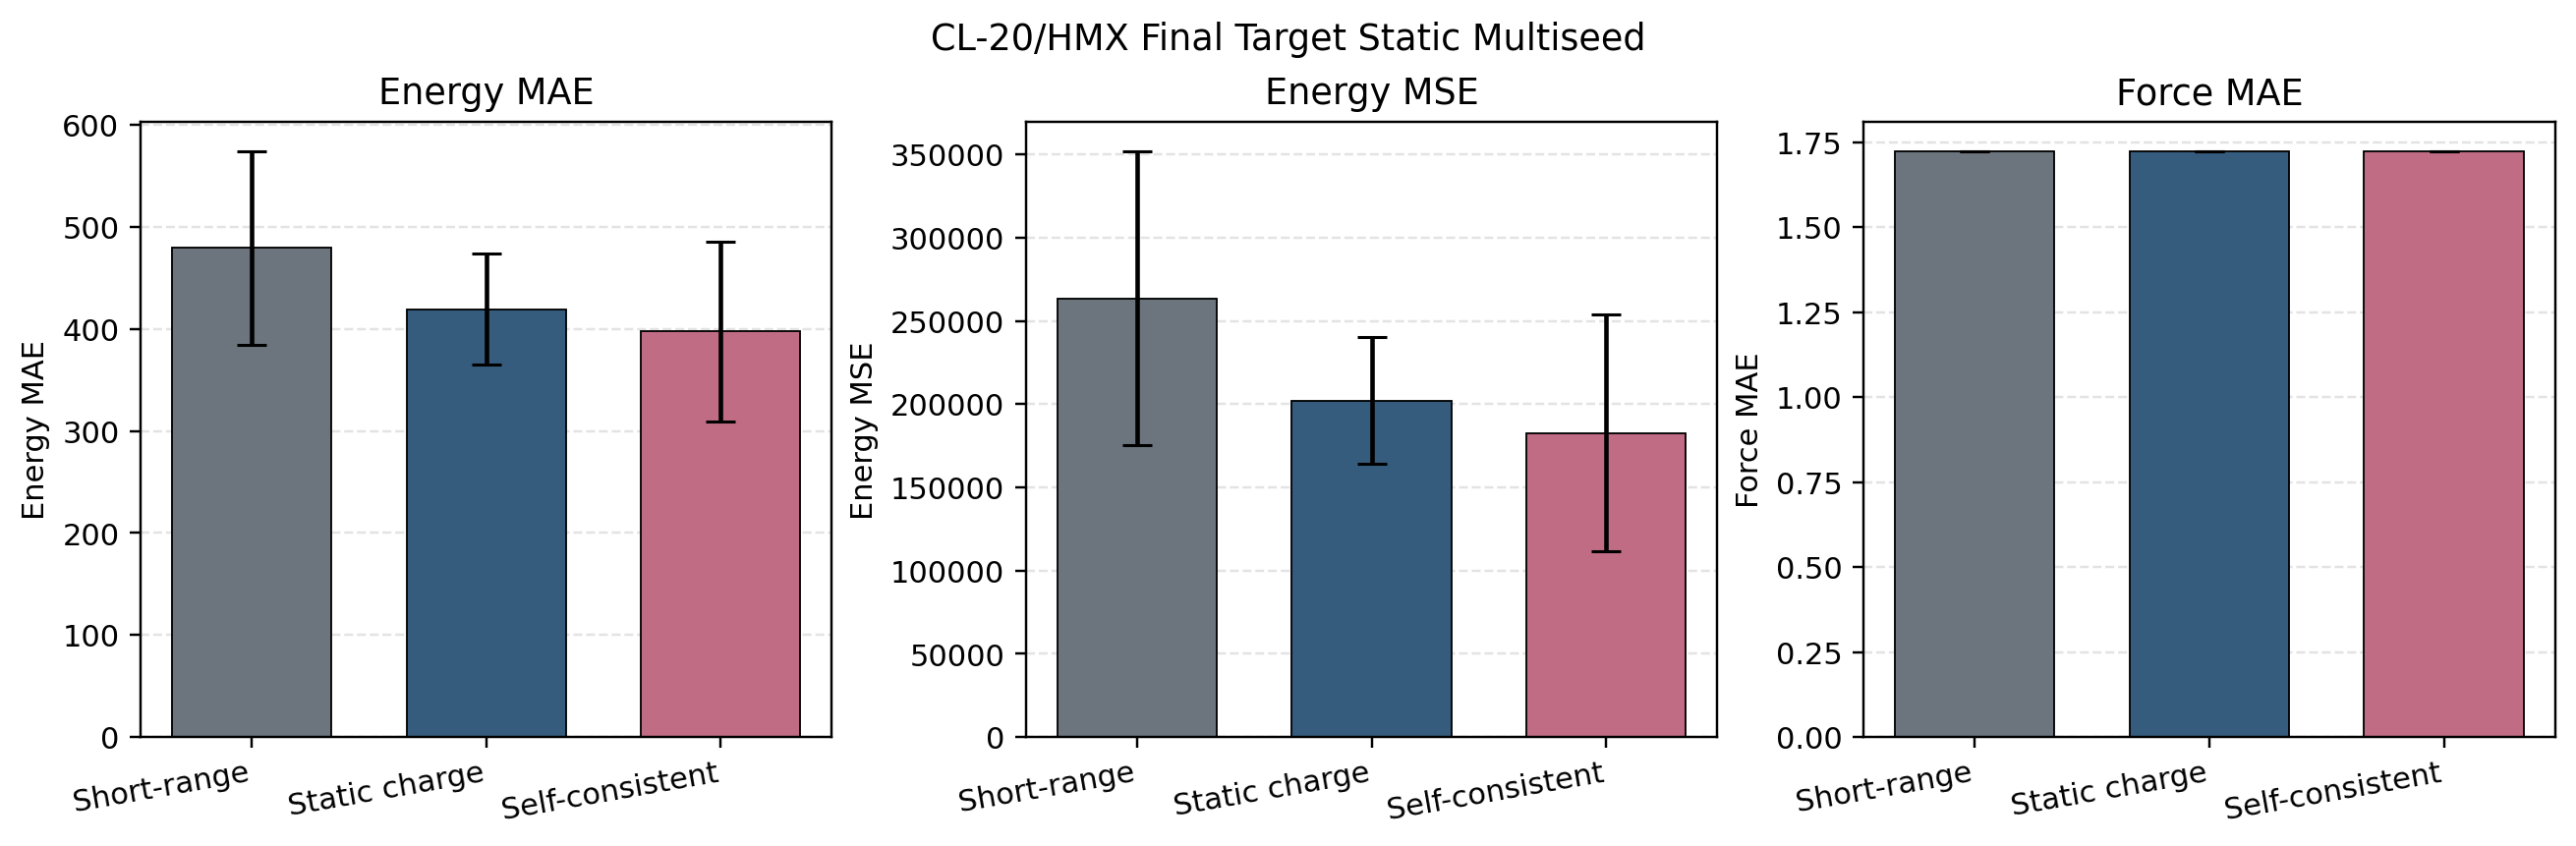
\includegraphics[width=0.92\linewidth]{figs/cl20_hmx_target_static_multiseed.png}
    \caption{CL-20/HMX final-target static multiseed comparison over seeds $42$ and $123$. The energy hierarchy is unambiguous on the energetic-material target: \texttt{self\_consistent} is best, \texttt{static\_charge} is second, and \texttt{short\_range} is weakest, while force MAE remains effectively tied.}
    \label{fig:cl20_hmx_target_static_multiseed}
\end{figure}

\begin{figure}[t]
    \centering
    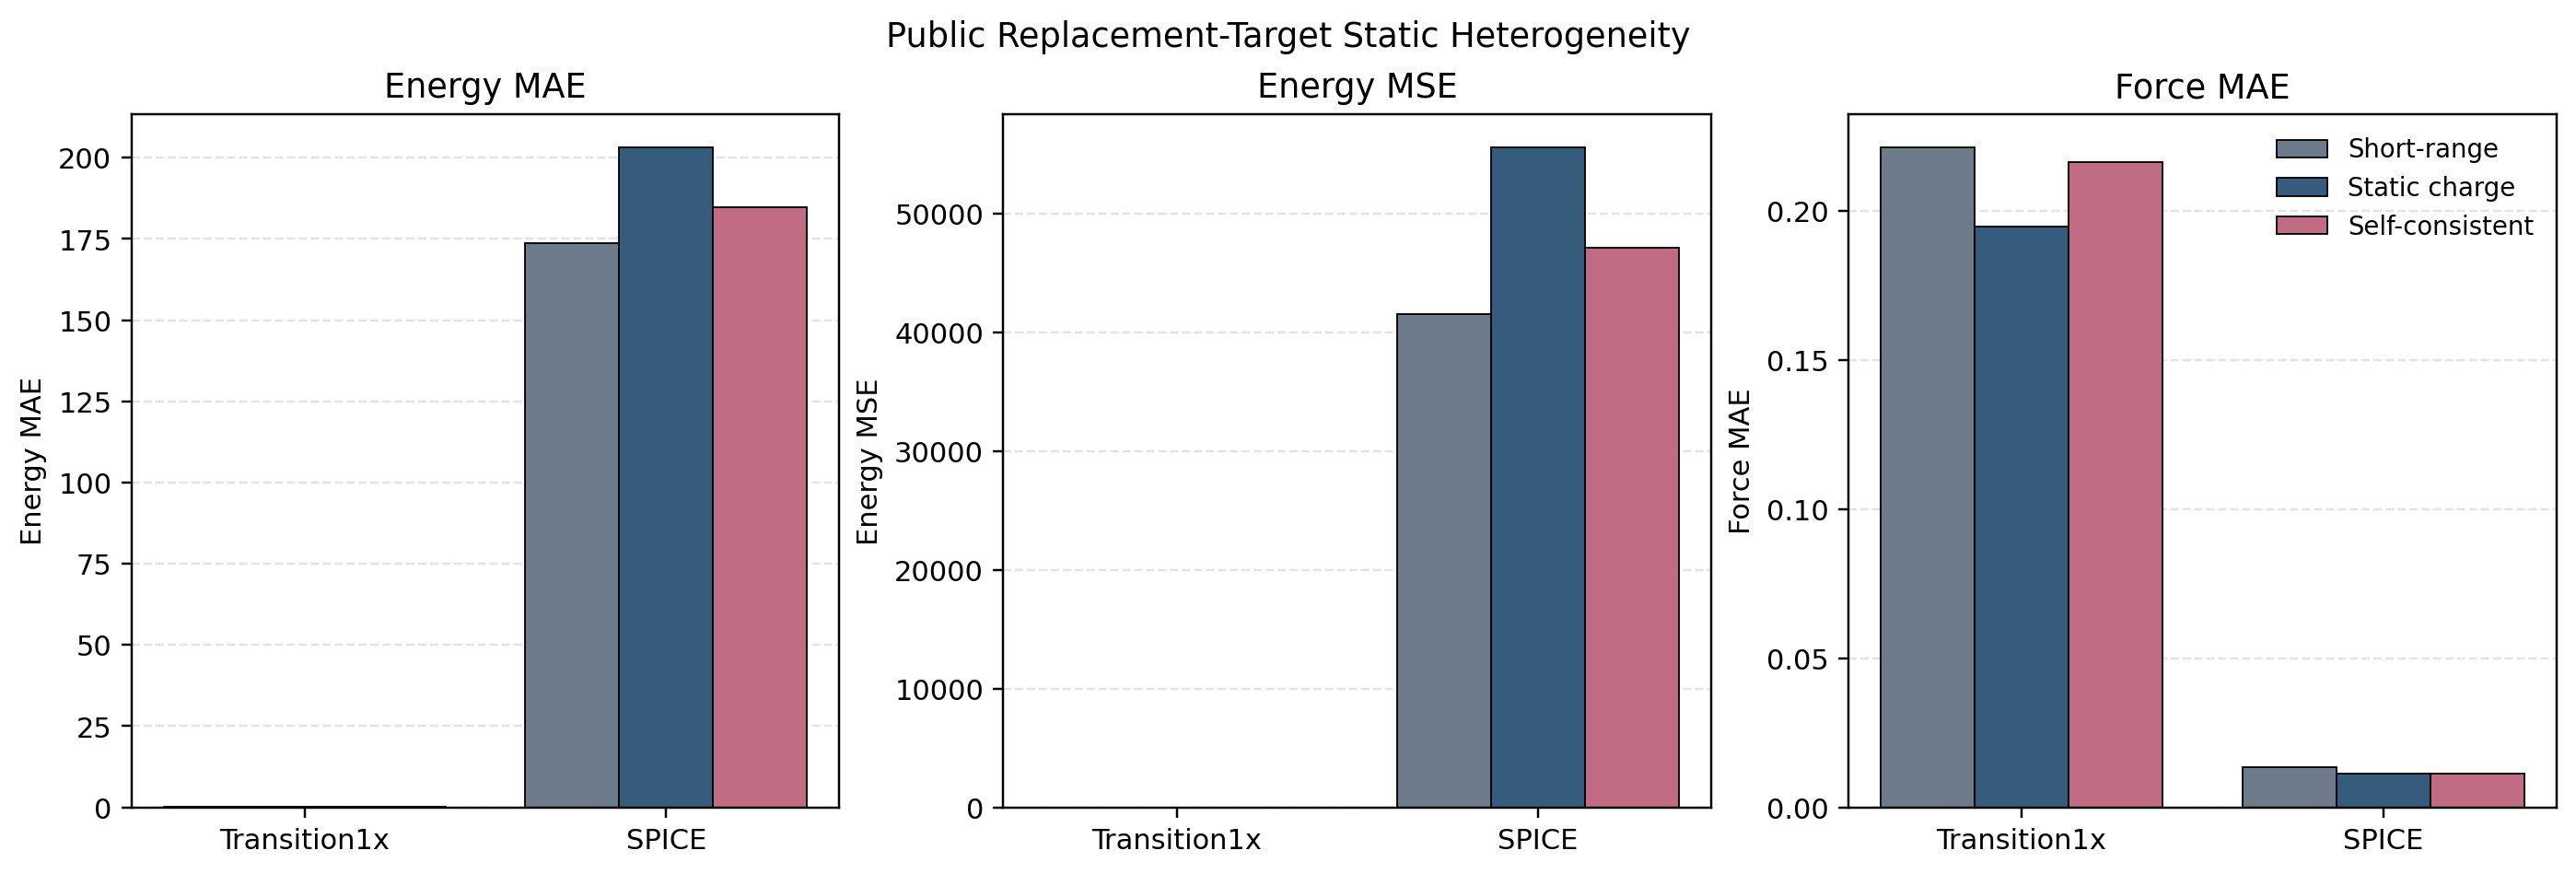
\includegraphics[width=\linewidth]{figs/replacement_target_static_summary.png}
    \caption{Static heterogeneity across the two public surrogate systems. Transition1x favors the charge-aware families overall, whereas SPICE favors \texttt{short\_range} on energy metrics but the charge-aware branches on force MAE.}
    \label{fig:replacement_target_static_summary}
\end{figure}

\begin{figure}[t]
    \centering
    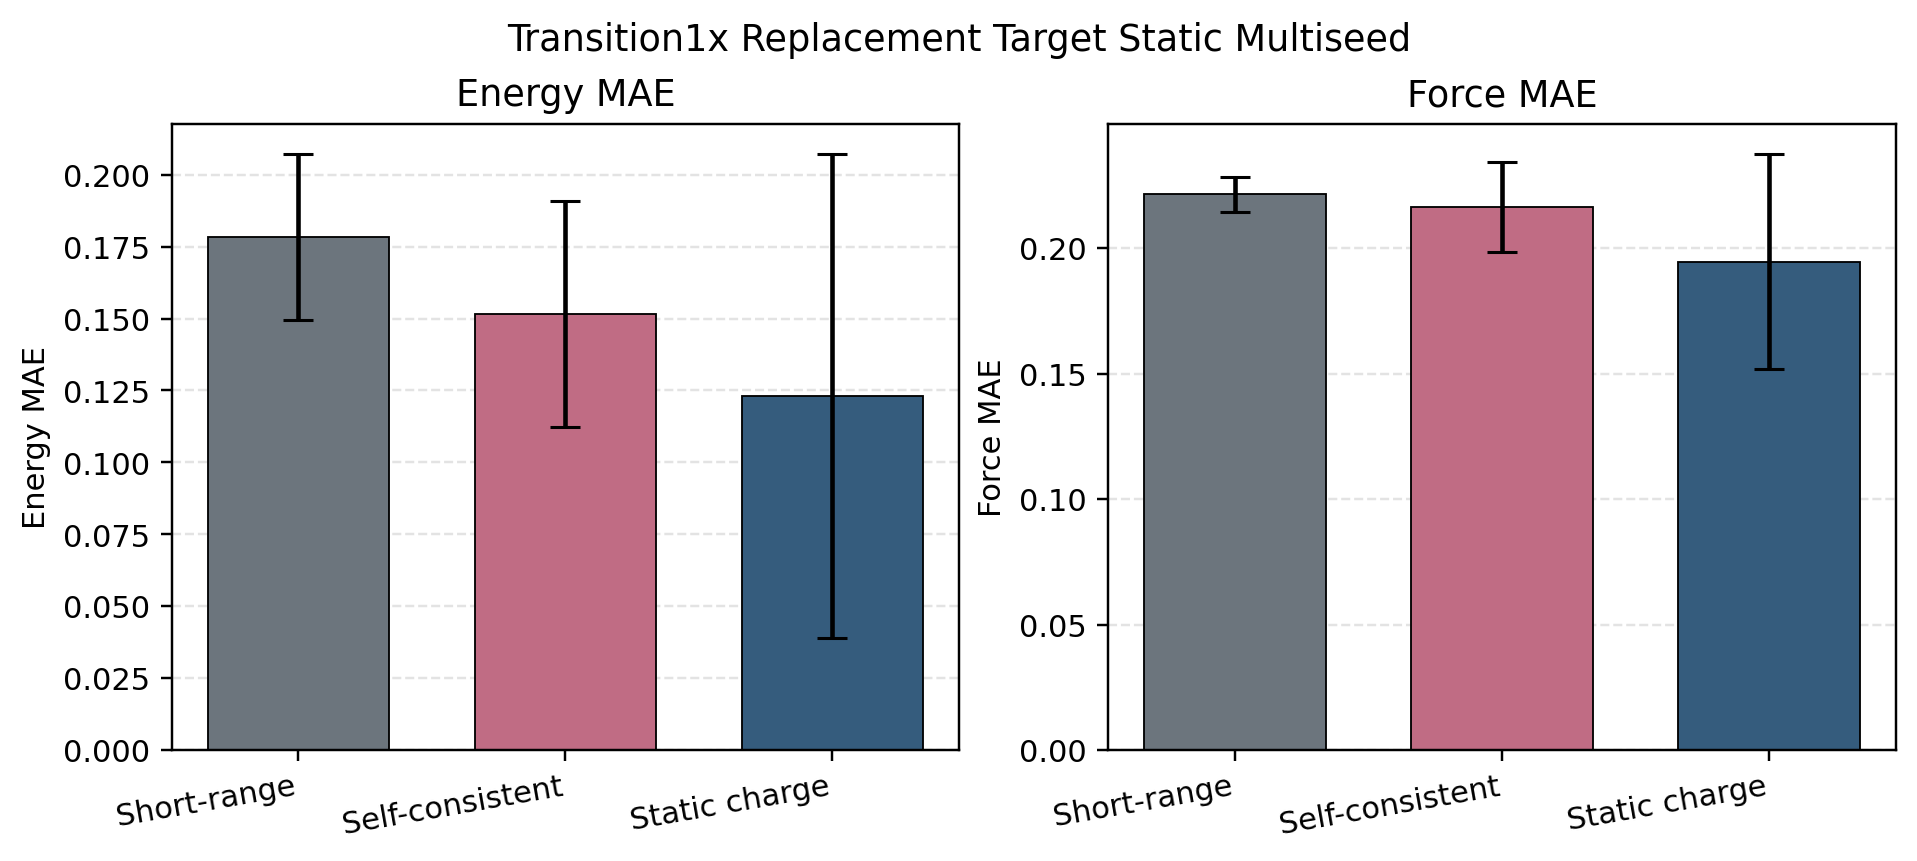
\includegraphics[width=0.92\linewidth]{figs/transition1x_target_static_multiseed.png}
    \caption{Transition1x static multiseed comparison over seeds $7$ and $123$. Both charge-aware variants outperform the short-range baseline, and \texttt{static\_charge} is the strongest overall family.}
    \label{fig:transition1x_target_static_multiseed}
\end{figure}

\begin{figure}[t]
    \centering
    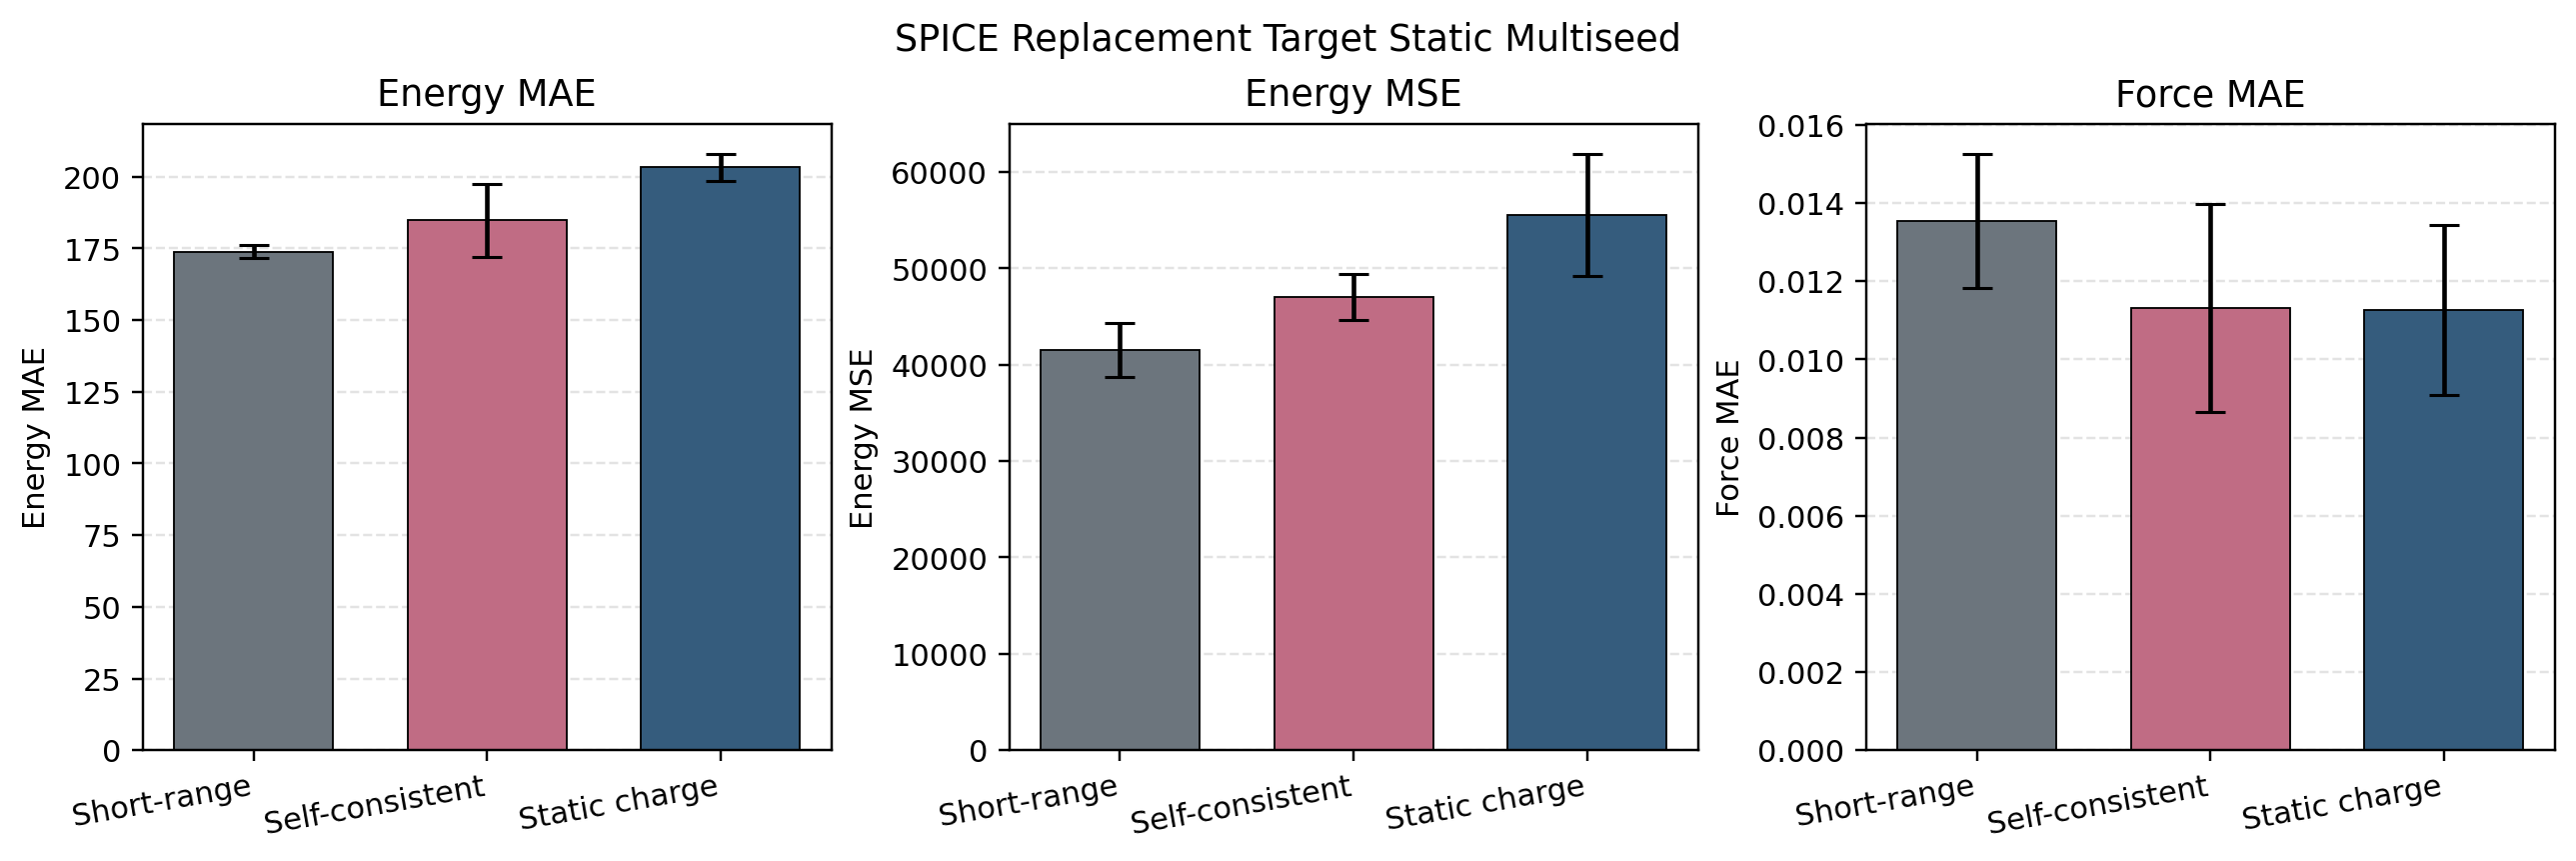
\includegraphics[width=0.92\linewidth]{figs/spice_target_static_multiseed.png}
    \caption{SPICE static multiseed comparison over seeds $7$ and $123$. \texttt{short\_range} is strongest on energy metrics, whereas both charge-aware branches improve force MAE and remain nearly tied.}
    \label{fig:spice_target_static_multiseed}
\end{figure}

\begin{figure}[t]
    \centering
    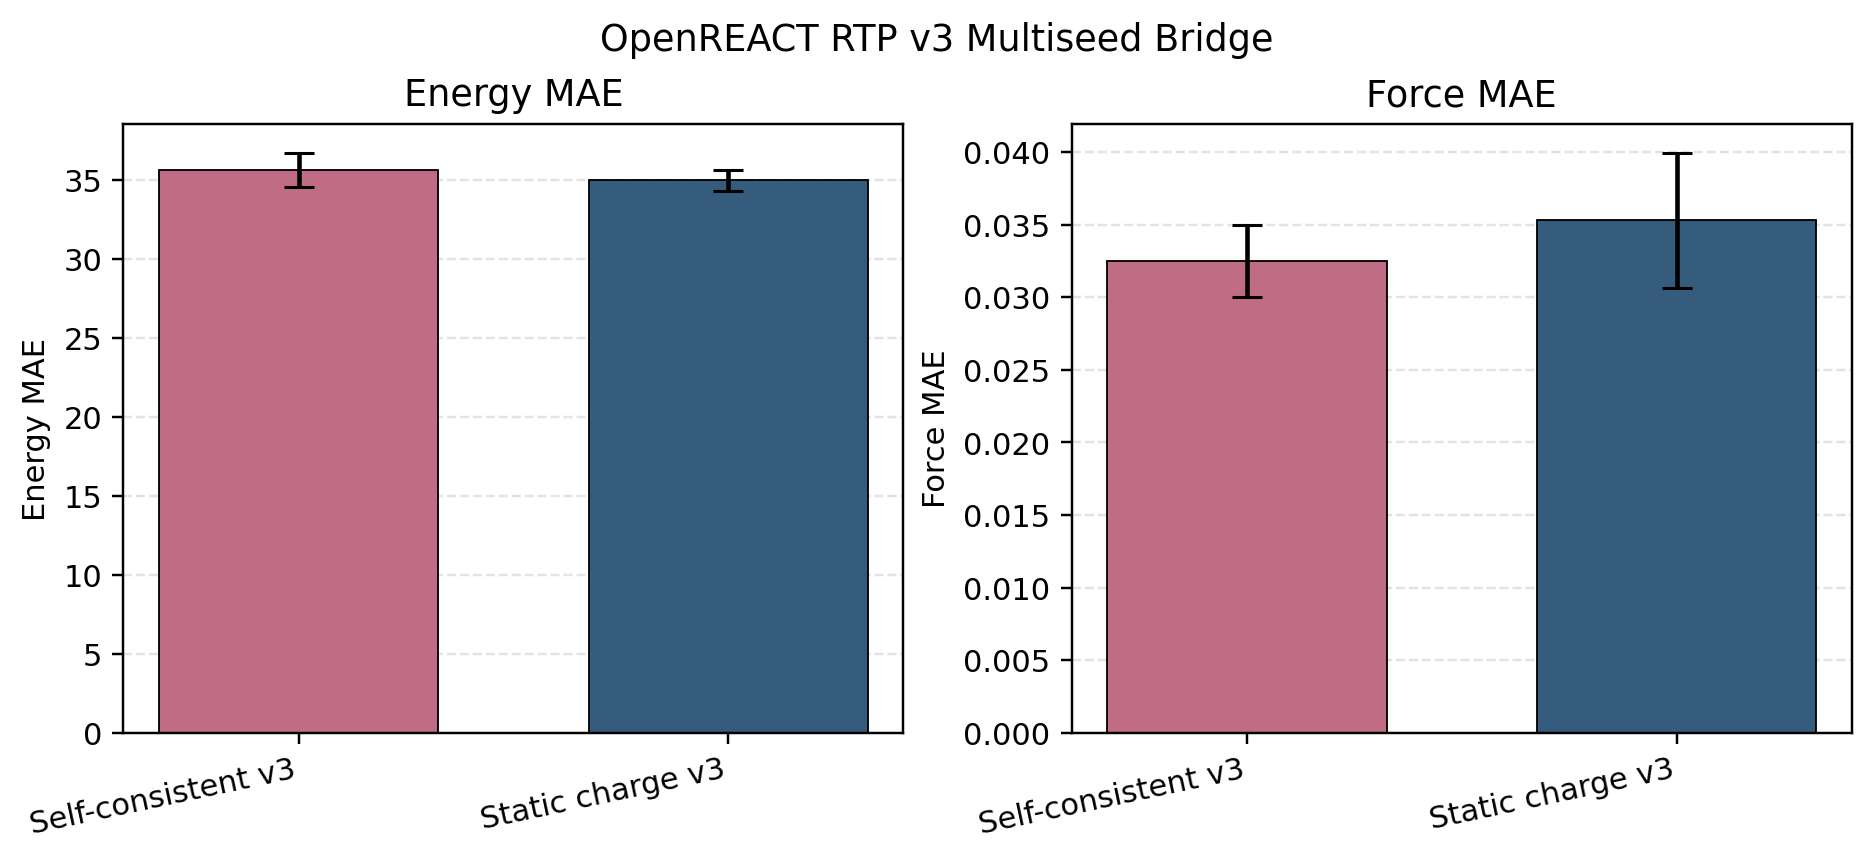
\includegraphics[width=0.92\linewidth]{figs/openreact_v3_multiseed_static.png}
    \caption{OpenREACT public reference system, conservative v3 multiseed comparison over seeds $7$ and $123$. The static-charge reference remains better on energy MAE, while the stabilized self-consistent branch improves force MAE.}
    \label{fig:openreact_v3_static}
\end{figure}

\subsection{Dynamical results}
\label{sec:results_dynamics}

The central dynamical question is whether self-consistent electrostatics change the failure modes of interatomic potentials under nonequilibrium trajectories. The evidence points to a mixed answer: charge-aware models can improve static ranking, but their dynamical effect remains strongly dependent on the target system and the stress protocol.

\subsection{Reference system stability: OpenREACT}
On the OpenREACT reference system, all model families, \texttt{short\_range}, \texttt{static\_charge}, and \texttt{self\_consistent}, remain numerically stable over short horizons ($300$ steps). Under the more demanding protocol ($2400$ steps at $\Delta t = 0.50$), the charge-aware branches show smaller potential-energy drift than the short-range baseline. The \texttt{static\_charge} and \texttt{self\_consistent} variants, however, remain nearly tied. Charge-aware dynamics are therefore active on the bridge system, while explicit self-consistency does not separate itself from a fixed-partial-charge reference in this regime.

\subsection{Hierarchy reversal: Transition1x}
Transition1x provides a stricter test of dynamical robustness. Although the static results in Section \ref{sec:results_static} favour the charge-aware families, the dynamical stress tests reverse that hierarchy. Under the harshest protocol, the \texttt{short\_range} baseline is substantially more stable than both charge-aware branches. For frames $64$ and $128$, the \texttt{short\_range} model never crosses the selected force or drift thresholds within the $2400$-step horizon, whereas both charge-aware branches cross them before step $2251$.

Bond-network observables clarify that reversal. The onset of local structural anomalies, measured by bond-threshold crossings and coordination-number reduction, is nearly synchronized across all three families. The divergence appears only in the post-onset regime: \texttt{short\_range} preserves a larger stability margin after the initial bond-network rearrangement, whereas the charge-aware families enter the degraded regime earlier. Electrostatic corrections therefore remain compatible with improved static force accuracy while still introducing additional sensitivity once the geometry becomes strongly distorted.

\subsection{Frame-selective synchronized collapse: SPICE}
SPICE reveals a different organization of failure. Unlike Transition1x, the SPICE trajectories do not show a clear family-level threshold hierarchy. Instead, the dominant signal is frame selectivity: on the most fragile trajectories, such as frame $64$, all three families undergo synchronized bond-network collapse by step $150$, whereas on more stable frames all families remain intact across the full horizon. For this system, the intrinsic susceptibility of specific trajectories to collective bond failure therefore dominates over inter-family differences in electrostatic representation.

\subsection{Final target plateau: CL-20/HMX}
The final energetic-material benchmark sharpens the main dynamical boundary. A sequence of progressively stronger protocols was applied to the CL-20/HMX data: short smoke trajectories, a longer horizon test, stress rollouts, threshold-aware stress, later-frame reaction-progress trajectories, a dense multiframe ensemble, and finally a focused key-bond survival comparison on the most sensitive frames. Across this ladder, the leading source of variation is the starting frame rather than the model family, and the new frame-versus-family dominance summary makes that statement quantitative rather than impressionistic.

The static hierarchy from Section \ref{sec:results_static} therefore does not propagate into a clear dynamical hierarchy under the current nonequilibrium protocols. In the threshold-aware stress analysis, all three families cross the potential-drift threshold at nearly identical times within each frame: around step $1631$ for frame $64$, around $1560$ for frame $128$, and around $1636$--$1637$ for frame $192$. Force and total-energy thresholds remain untriggered across this comparison.

The dense frame ensemble reinforces the same interpretation. Frames $32$, $64$, and $160$ are visibly more fragile than the others in molecular-integrity space, yet within a fixed frame the three families remain nearly indistinguishable.

The focused key-bond survival comparison gives the clearest chemical view of this boundary. On frame $32$, all three families finish with the same molecular-integrity fraction ($0.333$), the same retained C--N bond fraction ($0.910$), the same retained N--O bond fraction ($0.827$), and the same first molecular-integrity crossing below $0.5$ (step $390$), with the potential-drift threshold appearing at step $1117$--$1118$. Frame $64$ is similar: all three families end at molecular integrity $0.286$, retained C--N $0.912$, retained N--O $0.553$, and the same first integrity crossing at step $390$. Even on frame $160$, where the molecular-integrity crossing shifts earlier to step $360$--$370$, the family-level spread remains negligible (Figure \ref{fig:cl20_hmx_target_dynamics_keybond_survival}).

The dominance summary compresses that pattern into one quantitative comparison. For the final molecular-integrity and retained-bond endpoints, the mean spread across families within a fixed frame is exactly zero, while the same family's spread across frames reaches $0.464$ in final molecular integrity and $0.362$ in retained N--O fraction (Table \ref{tab:cl20_hmx_frame_family_dominance}). Even the event-onset metrics follow the same ordering: the mean spread across frames is about $8\times$ larger than the family spread for the first integrity crossing and about $184\times$ larger for the first drift-threshold step.

A dedicated multiseed nitro-focus analysis on frame $160$ sharpens the same point rather than reversing it. Averaged over $15$ variants spanning \texttt{short\_range}, \texttt{static\_charge}, \texttt{self\_consistent}, and two damped self-consistent ablations, the retained nitro N--O fraction is $0.444$ for \texttt{short\_range} and $0.463$ for every charge-aware family, while the nitro-motif integrity converges to the same mean value ($0.148$) for all five families and the first motif-integrity crossing below $0.5$ remains tightly clustered around steps $1647$--$1663$.

We also tested two stronger charge-aware modifications targeted directly at this boundary: a train-matched self-consistent comparison that removes the rollout-time damping used in the earlier horizon test, plus a stability-gated adaptive branch that modulates the self-consistent update step size on the fly. The train-matched comparison is especially important because it closes the most obvious method objection.

On frame $160$, restoring the static-side self-consistent settings (\texttt{charge\_iterations} $=4$, full-step updates, no rollout-only gate) does not create a new family-level win. Instead, it leaves the main endpoint picture essentially unchanged while shifting the onset metrics only modestly: the first potential-drift threshold moves from step $1067$ in the rollout-stabilized self-consistent family to step $1058$ in the train-matched family, the final molecular-integrity fraction remains $0.583$ in both cases, and retained N--O fraction changes slightly from $0.903$ to $0.887$. The same train-matched comparison also advances the first $0.70$ bond-threshold crossing from $433.3$ to $363.3$, which weakens rather than strengthens the hypothesis that the earlier negative result was caused purely by rollout-time damping.

In other words, the absence of a family-level dynamic gain survives the most direct configuration-fairness check we can presently perform on the fragile-frame target.

The new fragile-frame analysis makes the remaining dynamic signal more specific. The earlier failure-manifold comparison showed that the train-matched branch was the only self-consistent variant with any clear positive signal on the real target, but the denser failure-window analysis around frames $56$, $64$, and $72$ changes the interpretation of that signal.

This denser comparison rejects a broad onset-gain story: averaged over five seeds, train-matched \texttt{self\_consistent} reaches the first $0.70$ bond-threshold crossing earlier than \texttt{static\_charge} on all three frames ($-12$ steps on frame $56$, $-34$ on frame $64$, and $-18$ on frame $72$). The positive signal instead reorganizes around endpoint survival.

On frame $64$, train-matched \texttt{self\_consistent} still improves the final molecular-integrity fraction from about $0.343$ for \texttt{static\_charge} to about $0.426$, and on frame $72$ it improves final molecular integrity from about $0.774$ to about $0.832$ while also delaying the first integrity crossing by about $195$ steps and slightly improving final nitro N--O survival. Frame $56$ remains unfavorable, with train-matched \texttt{self\_consistent} worse than \texttt{static\_charge} on final integrity and nitro survival.

Figure \ref{fig:cl20_hmx_failure_window} and Table \ref{tab:cl20_hmx_failure_window} compress that result into the most direct comparison. The clearest local gain is frame $72$, where the train-matched branch improves final integrity relative to both \texttt{static\_charge} and \texttt{short\_range}, while frame $64$ still shows a smaller endpoint gain and frame $56$ shows no gain at all. The fragile-window analysis therefore sharpens the dynamic conclusion in a more constructive way than the earlier broad ladders alone: on the real CL-20/HMX target, the strongest positive signal is not a generic onset delay but a narrow endpoint-survival gain window around frames $64$--$72$.

Even this stronger window remains local rather than global, because it does not extend across the broader fragile manifold and does not establish a robust family-level hierarchy over the final target as a whole.

The adaptive-gated branch remains informative for a different reason. On the same frame-$160$ horizon test, neither gated modification improves the existing charge-aware drift-threshold plateau in a meaningful structural sense, and the adaptive-gated variant preserves the same molecular-integrity outcome while entering a substantially more expensive rollout regime.

A matched profiled comparison now makes the family-level cost ordering explicit on that frame: \texttt{short\_range}, \texttt{static\_charge}, and train-matched \texttt{self\_consistent} all remain within the same early-event band, while rollout costs still rise from about $20$ s to $42$ s to $112$ s before the adaptive-gated branch reaches about $190$ s without creating a better endpoint hierarchy (Figure \ref{fig:cl20_hmx_target_adaptive_gate_cost}).

The submission package includes a dedicated QEq-versus-failure bridge table, a frame-versus-family dominance summary, a train-matched frame-$160$ dynamics table, a frame-$160$ adaptive-gate cost-versus-outcome table, a threshold-aware fragile-frame summary, and a failure-manifold summary to make the implication explicit: the charge-aware branches remain measurably active in the static diagnostics, yet within a fixed CL-20/HMX frame the dominant variation in final integrity and key-bond survival still comes from frame choice rather than from family choice, while progressively more elaborate charge-aware branches can impose progressively larger rollout cost without producing a new event hierarchy or a better structure-survival endpoint.

The real target therefore supports a stronger statement than drift alone would allow: key-bond survival, nitro-motif survival, and fragment-level integrity remain dominated by frame selection rather than by the choice among \texttt{short\_range}, \texttt{static\_charge}, and \texttt{self\_consistent}, even though the train-matched branch can open a narrow local endpoint-survival gain window on the most fragile frames.

\subsection{Summary of dynamical findings}
Taken together, the dynamical evidence defines a clear boundary for charge-self-consistent potentials. The public systems support a measurable electrostatic effect and substantial heterogeneity across surrogate targets, but they do not support a universal dynamical improvement. Transition1x shows that charge-aware families can become less stable than the short-range baseline after comparable early rearrangement, whereas SPICE shows that some trajectories collapse synchronously across all three families before any hierarchy can emerge. The final CL-20/HMX benchmark goes further: under the present nonequilibrium protocols, degradation is primarily frame-dependent rather than family-dependent, even when evaluated by key-bond survival and molecular-integrity observables. These findings support CSC-MACE as a physically motivated architecture while defining the stabilization problem that remains unresolved on the final target.

\begin{figure}[t]
    \centering
    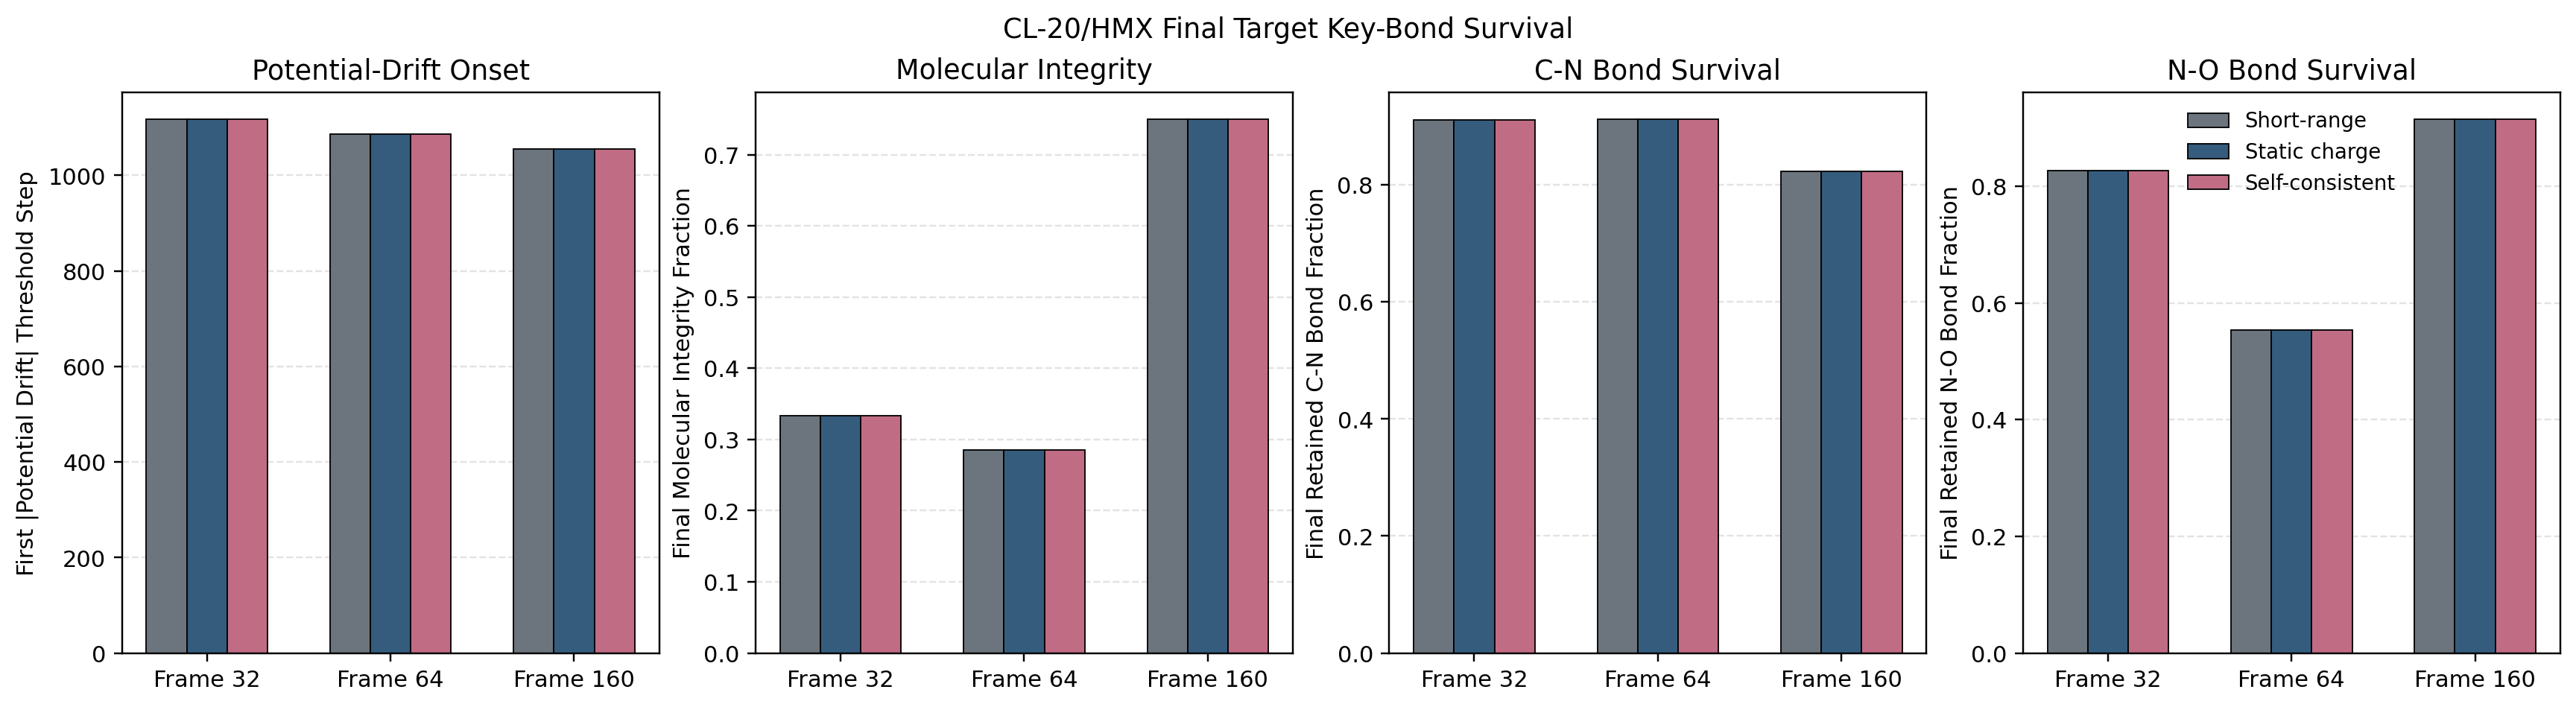
\includegraphics[width=\linewidth]{figs/cl20_hmx_target_dynamics_keybond_survival.png}
    \caption{CL-20/HMX final-target focused key-bond survival comparison on the most sensitive frames $32$, $64$, and $160$. Potential-drift onset, molecular integrity, and C--N / N--O bond-family survival all vary substantially across starting frames, but remain nearly unchanged across the three model families within each frame.}
    \label{fig:cl20_hmx_target_dynamics_keybond_survival}
\end{figure}

\input{../results/target/cl20_hmx_frame_family_dominance.tex}

\begin{figure}[t]
    \centering
    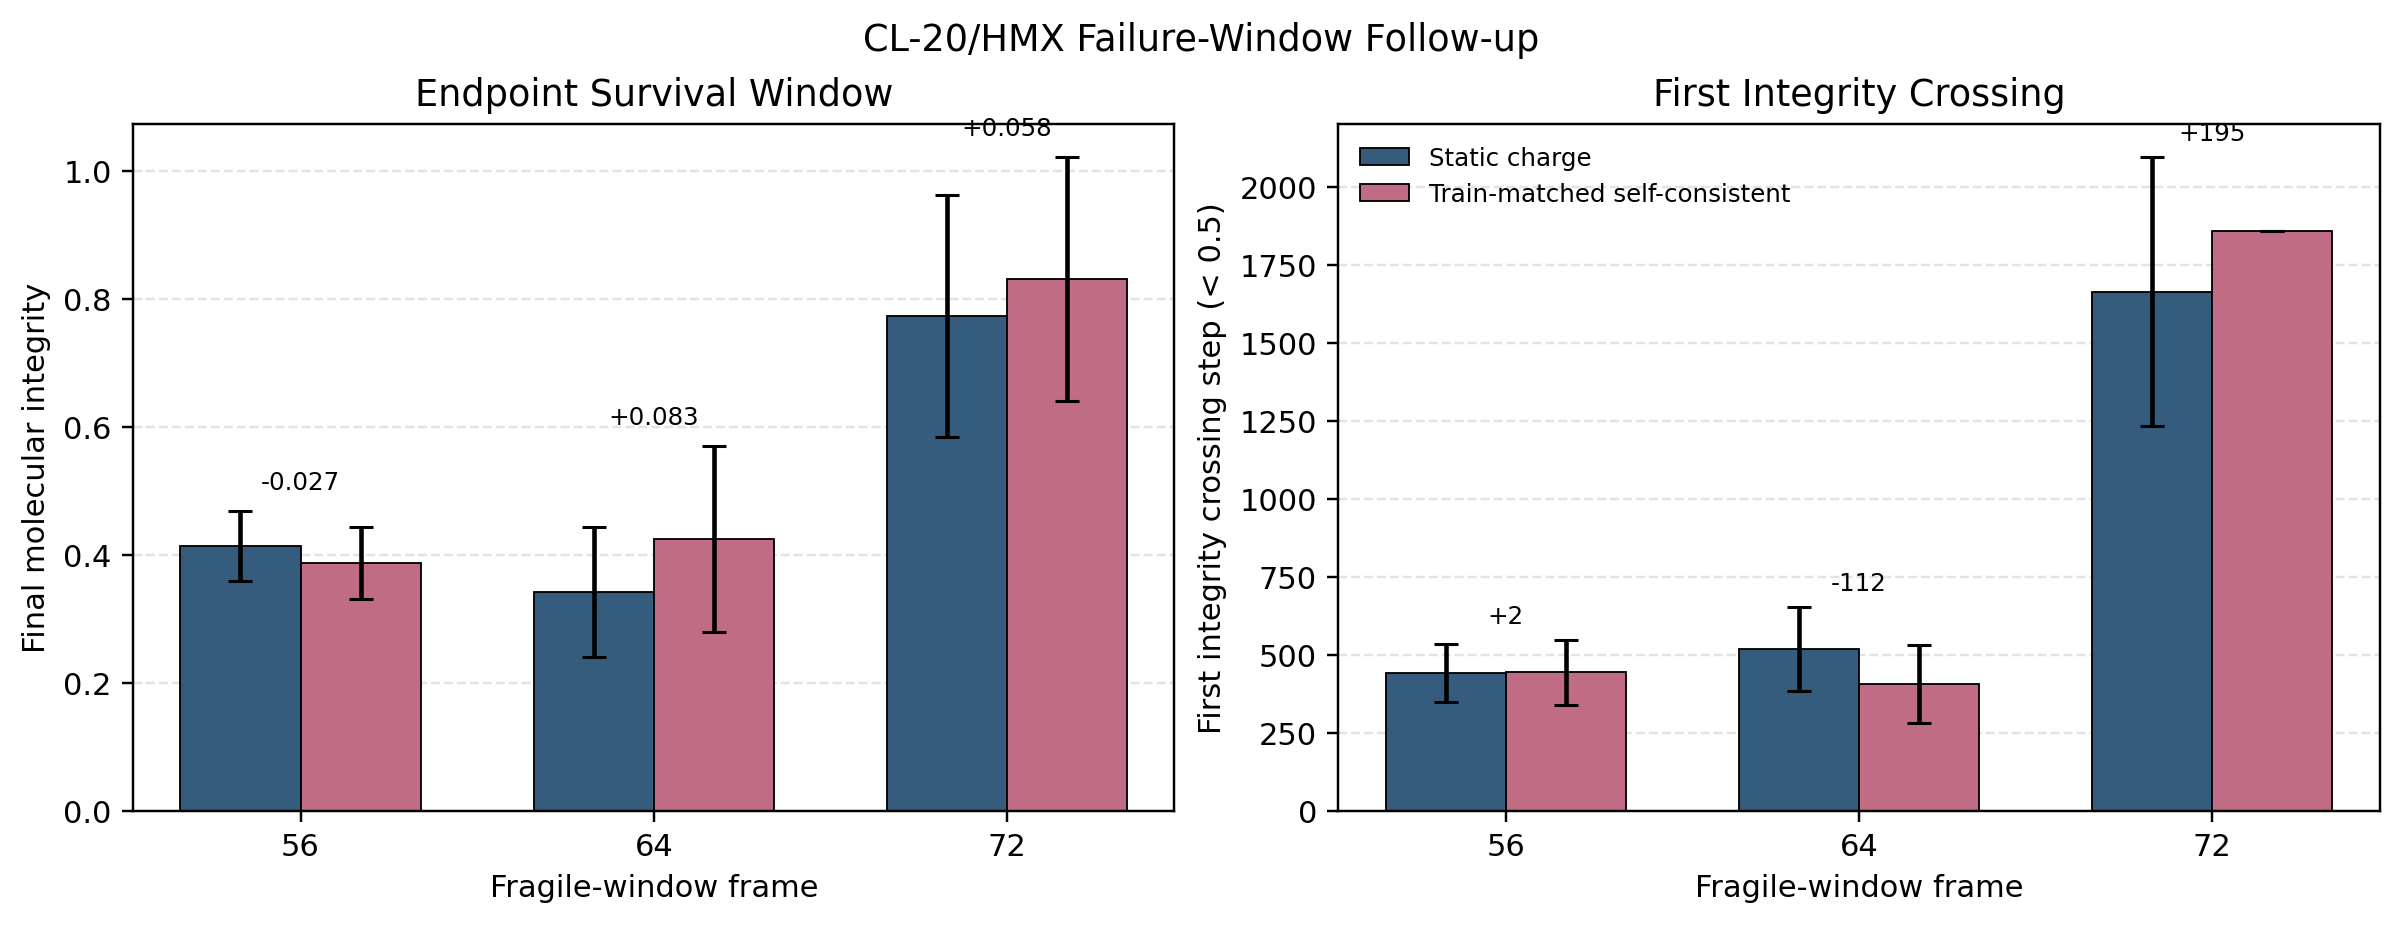
\includegraphics[width=\linewidth]{figs/cl20_hmx_failure_window.png}
    \caption{Dense CL-20/HMX fragile-window analysis comparing \texttt{static\_charge} against train-matched \texttt{self\_consistent}. The positive dynamic signal is not a broad onset advantage. Instead, endpoint survival improves only in a narrow local window: frame $56$ remains unfavorable, frame $64$ shows a modest final-integrity gain, and frame $72$ shows the clearest combined endpoint benefit.}
    \label{fig:cl20_hmx_failure_window}
\end{figure}

\input{../results/target/cl20_hmx_failure_window_summary.tex}

\begin{figure}[t]
    \centering
    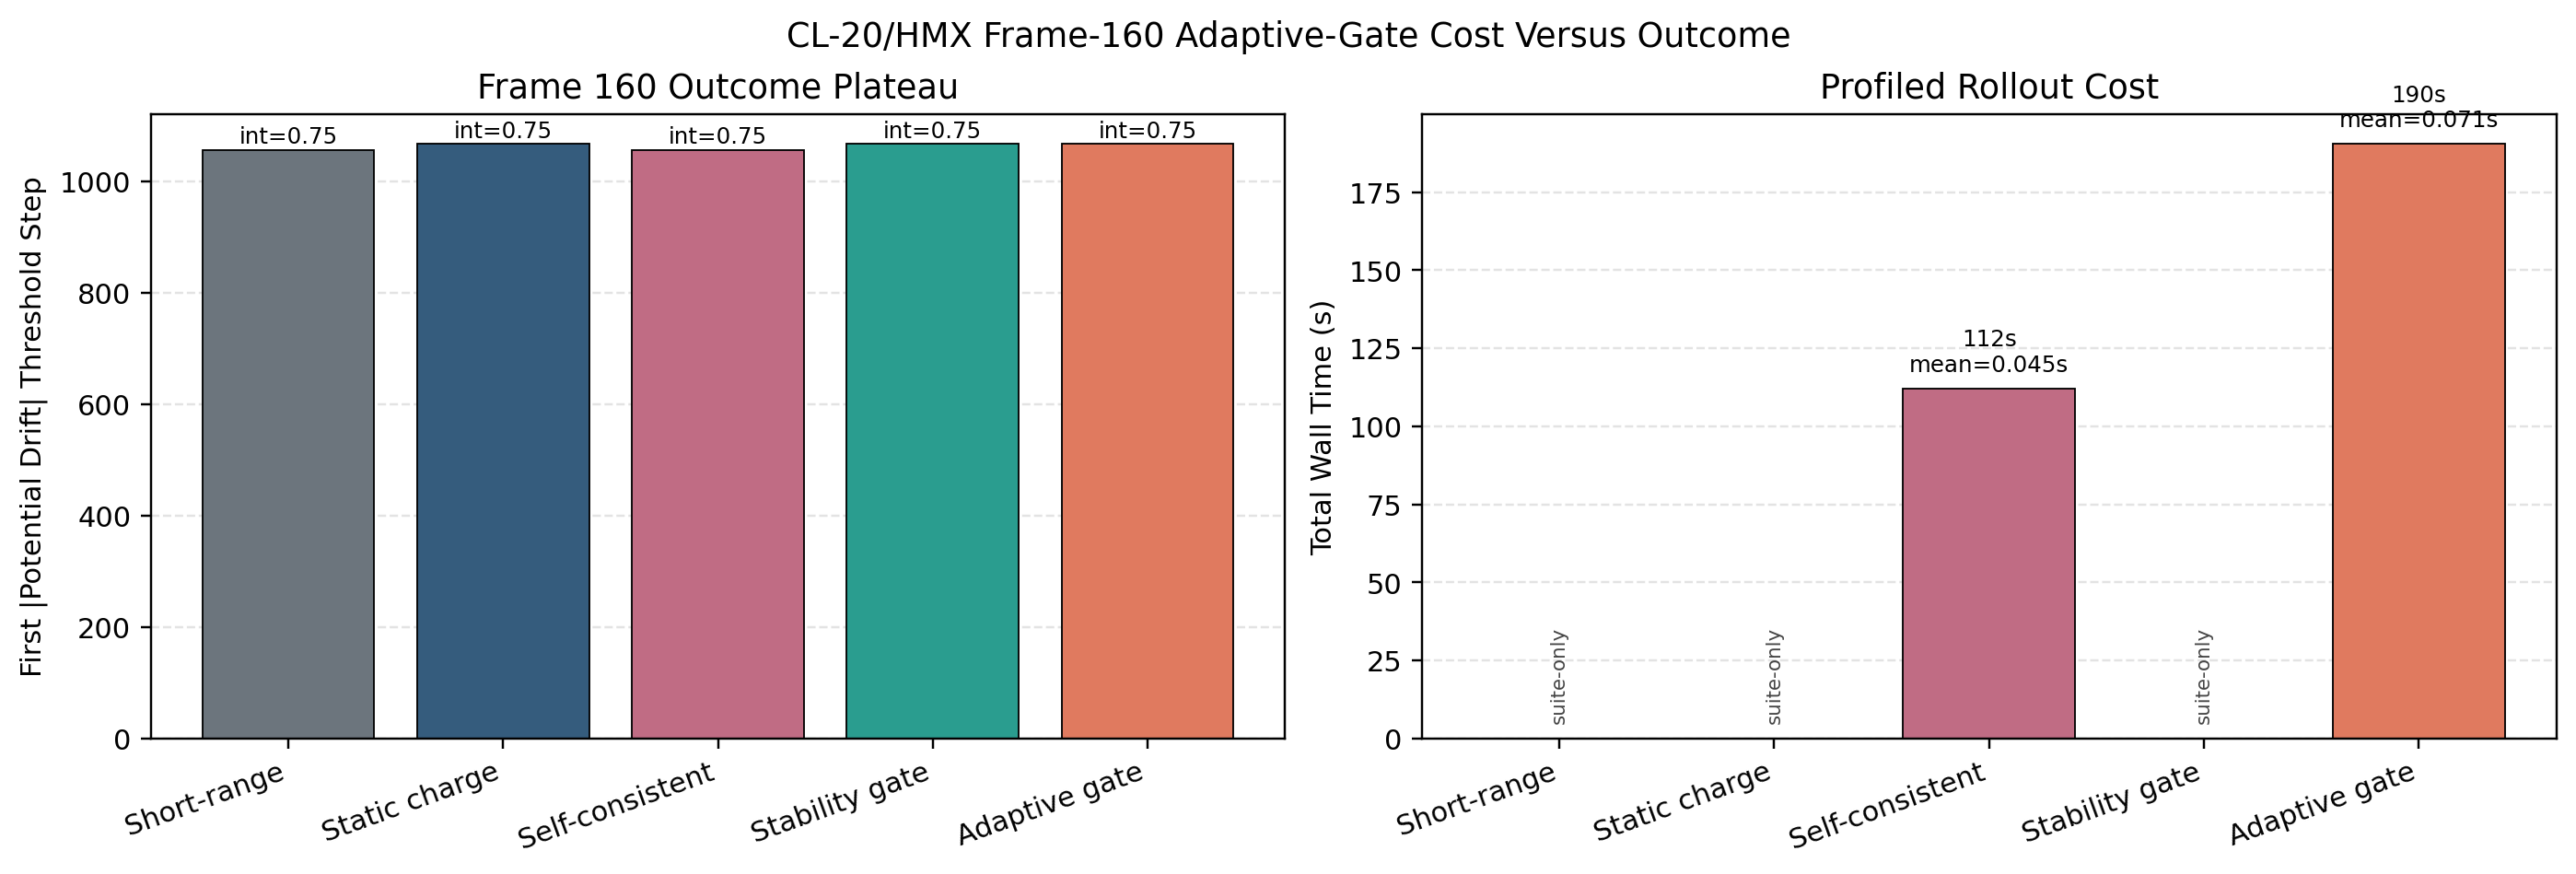
\includegraphics[width=0.95\linewidth]{figs/cl20_hmx_adaptive_gate_cost.png}
    \caption{CL-20/HMX frame-$160$ cost-versus-outcome comparison for the breakthrough charge-aware branches. The stronger gated variants recover the same structure-level outcome and the same charge-aware drift-threshold plateau, but the adaptive-gated branch does so at substantially higher rollout cost than the plain self-consistent branch.}
    \label{fig:cl20_hmx_target_adaptive_gate_cost}
\end{figure}

\section{Discussion}
\label{sec:discussion}

The discussion is most useful when three questions are separated: what explicit self-consistency adds beyond simpler charge-aware corrections in static fitting, how that increment behaves once trajectories leave the near-equilibrium manifold, and what the final CL-20/HMX target implies about the present scope of charge-aware stabilization.

We ablate the self-consistent charge-equilibration module by comparing full CSC-MACE against \texttt{static\_charge}, where the equivariant features predict a simpler non-self-consistent charge correction, and \texttt{short\_range}, which excludes explicit electrostatics entirely. On OpenREACT, the self-consistent branch achieves a mean force MAE of $3.25 \times 10^{-2} \pm 2.49 \times 10^{-3}$, improving on both alternatives, but this force gain is accompanied by a slight energy penalty relative to \texttt{static\_charge}.

That tradeoff is methodologically informative because it shows that explicit self-consistency is not redundant with a simpler charge-aware head. The persistent energy--force split indicates that self-consistency captures higher-order field response, while the present parameterization leaves room for tighter coupling between the electrostatic and short-range terms.

The Transition1x stress tests reveal the first clear limitation of that increment: static gains of the charge-aware models do not translate directly into enhanced trajectory stability under extreme shock protocols. All families synchronize at the onset of local bond-network rearrangement, but the \texttt{short\_range} baseline preserves a larger post-onset stability margin, whereas both charge-aware branches enter the degraded regime earlier. This suggests that the added electrostatic degrees of freedom, while physically useful near equilibrium, may introduce additional sensitivity in the highly distorted configurations characteristic of post-onset shock dynamics.

The real CL-20/HMX benchmark reveals a different and more decisive limitation. Static energy ranking improves monotonically from \texttt{short\_range} to \texttt{static\_charge} to \texttt{self\_consistent}, but that hierarchy does not produce a corresponding nonequilibrium separation under the current rollout protocols. Across stress, threshold-aware stress, reaction-progress trajectories, dense frame ensembles, and focused key-bond survival comparisons, the dominant variation is the starting frame rather than the model family.

In particular, molecular-integrity loss and C--N / N--O survival remain almost identical across the three families once the frame is fixed, while the same family's spread across frames is much larger. The focused dominance summary makes that point explicit: on the final key-bond analysis, the mean spread across families within a fixed frame is zero for the final molecular-integrity and retained-bond endpoints, whereas the frame-driven spread is about $8\times$ larger for the first integrity crossing and about $184\times$ larger for the first drift-threshold step.

A dedicated frame-$160$ nitro-focus multiseed analysis strengthens this limitation rather than weakening it: \texttt{short\_range} retains a mean nitro N--O fraction of $0.444$, whereas \texttt{static\_charge}, \texttt{self\_consistent}, and two damped self-consistent ablations all cluster at $0.463$; meanwhile, the nitro-motif integrity converges to the same mean value ($0.148$) across all five families, with first motif-integrity threshold crossings confined to the narrow band of steps $1647$--$1663$.

We then probed a stronger methodological intervention: a stability-gated self-consistent branch and an adaptive-gated branch that modulates the self-consistent mixing step size. On frame $160$, neither created a new family-level outcome beyond the simpler charge-aware plateau at step $1067$, and matched profiling shows a clear rollout-cost ordering on that same frame, from about $20$ s for \texttt{short\_range} to $42$ s for \texttt{static\_charge} to $112$ s for \texttt{self\_consistent}, before the adaptive-gated branch rises to about $190$ s while preserving the same key structure-survival outcome.

The practical boundary is therefore stronger than a simple reversal of static gain. On the final target, current CSC-MACE variants do not convert their static energy advantage into a reliably distinguishable dynamical event hierarchy, and more elaborate charge-aware updates can substantially increase computational burden without yielding a new structure-level advantage.

We emphasize that the effective charges predicted by CSC-MACE are parameters of a self-consistent interatomic potential and should not be over-interpreted as unique physical observables equivalent to any single DFT population analysis scheme such as Mulliken or Bader. Their primary role here is to improve force-field fidelity through the inclusion of long-range electrostatics. Recent charge-aware architectures have reached similar conclusions in adjacent settings: explicit charge degrees of freedom can be made active, interpretable, and useful, while the transfer of that information to non-equilibrium stability remains system-dependent \cite{fuchs2025celli,jung2026charge}. Whether closer alignment with explicit electronic-density observables would stabilize long-horizon dynamics remains an open question.

Taken together, these results argue for a layered validation strategy in which static error, early structural onset, fragment integrity, and post-onset stability are treated as distinct targets rather than interchangeable summaries. For energetic molecular crystals, the present CSC-MACE variants improve static energetics on the real target, but they do not induce a corresponding family-level separation in the tested nonequilibrium event metrics.

Even stronger adaptive interventions tested directly on the most fragile CL-20/HMX frame only recover the existing charge-aware drift-threshold plateau while increasing rollout cost, showing that more adaptive self-consistency alone does not create a new dynamical hierarchy. The paper therefore defines a method boundary with unusual specificity: explicit self-consistency is active, measurable, and beneficial for the real-target static hierarchy, but its extra physical structure does not dominate the present nonequilibrium outcome.

The next challenge is therefore sharply defined: stabilize the electrostatic gain so that it propagates into dynamically relevant observables without disproportionate computational overhead. The current data boundary is equally clear: the CL-20/HMX release already supports a real force-labeled energetic-material benchmark, and a held-out HMX-only split table can now be regenerated from the GPU multiseed static analysis, but the present contiguous split still does not provide simultaneous held-out CL-20 and HMX coverage or the reviewer-complete thermodynamic and labeling provenance needed for a final pressure- or trajectory-history-resolved mechanistic decomposition.


\section*{Data availability}
The benchmark manifests, split definitions, cached analysis artifacts, figure-generation outputs, and target-benchmark provenance notes used in this study are included in the reproducibility package associated with this manuscript. The final CL-20/HMX benchmark file used here is traceable to two named upstream DeepMD-format packages recovered in the local workspace snapshot, as documented in the target-data provenance note. Because the current packaged release does not yet include a reviewer-complete upstream metadata record, access to the underlying staged arrays and to any later enriched metadata release should be coordinated through the corresponding author and the data-owning collaboration.

\section*{Code availability}
All training, evaluation, charge-equilibration, and rollout-analysis code required to reproduce the reported CSC-MACE results is included in the OpenClaw-based project repository associated with this manuscript. A manuscript-facing reviewer package containing the scripts, cached summaries, and plotting utilities used for the submitted figures and tables is available from the corresponding author upon reasonable request.

\section*{Author contributions}
Xiaohua Liu conceived the study, performed the model development and benchmark analysis, and drafted the manuscript. Dongping Chen contributed the CL-20/HMX data lineage clarification, target-benchmark curation guidance, and manuscript revision. Chengkai Zhang contributed to manuscript revision and benchmark discussion. Hongqian Sang contributed to manuscript revision and benchmark discussion. All authors reviewed and approved the manuscript.

\section*{Competing interests}
The authors declare no competing interests.

\bibliographystyle{plain}
\bibliography{refs}

\end{document}
